\chapter{Overview of the Approach}
\markboth{Overview of the Approach}{Overview of the Approach}
\label{chapter:ThesisOverview}


%%%%%%%%%%%%%%%%%%%%%%%%%%%%%%%%%%%%%%%%%%%%%%%%%%%%%%%%%%%%%%%%%%%%%%%%%%%%%%%%%%%%%%%%%%%%%%%%%%%%%%%%%%%%%%%%%%%%

In playing a music instrument, the musician establishes a more or less continuous interaction with the instrument. This interaction is based on complex mechanisms, allowing the fine-tuning of the sound-producing gestures via sensorimotor loops, including audio, visual and gestural feedbacks. Moreover, these sensory informations are directly influenced by the semantic information contained in the musical phrases, and may change the motor commands that produce the gesture. Virtual musical instruments controlled by natural gestures try to realistically reproduce this sensorimotor situation with the aim of approaching real instrumental situations.\\

Our work exploits the fact that there is a lack of knowledge on significant gestural characteristics for controlling virtual instruments producing sound. Especially when considering percussion gestures, preparatory and retraction gestures are considered as key components of music playing \citeIPA{dahl:AAA04}. In this thesis, we propose to go further and introduce a complete modeling of gesture, by designing a human-like character endowed with realistic and expressive behaviors. We particularly focus on the animation of virtual percussionists interacting with sound synthesis processes. Our approach is presented in \myfigname \ref{fig:thesisOverview}, showing the analysis-synthesis methodology adopted for synthesizing percussion performances.

\begin{figure}%[H]
	\begin{center}
		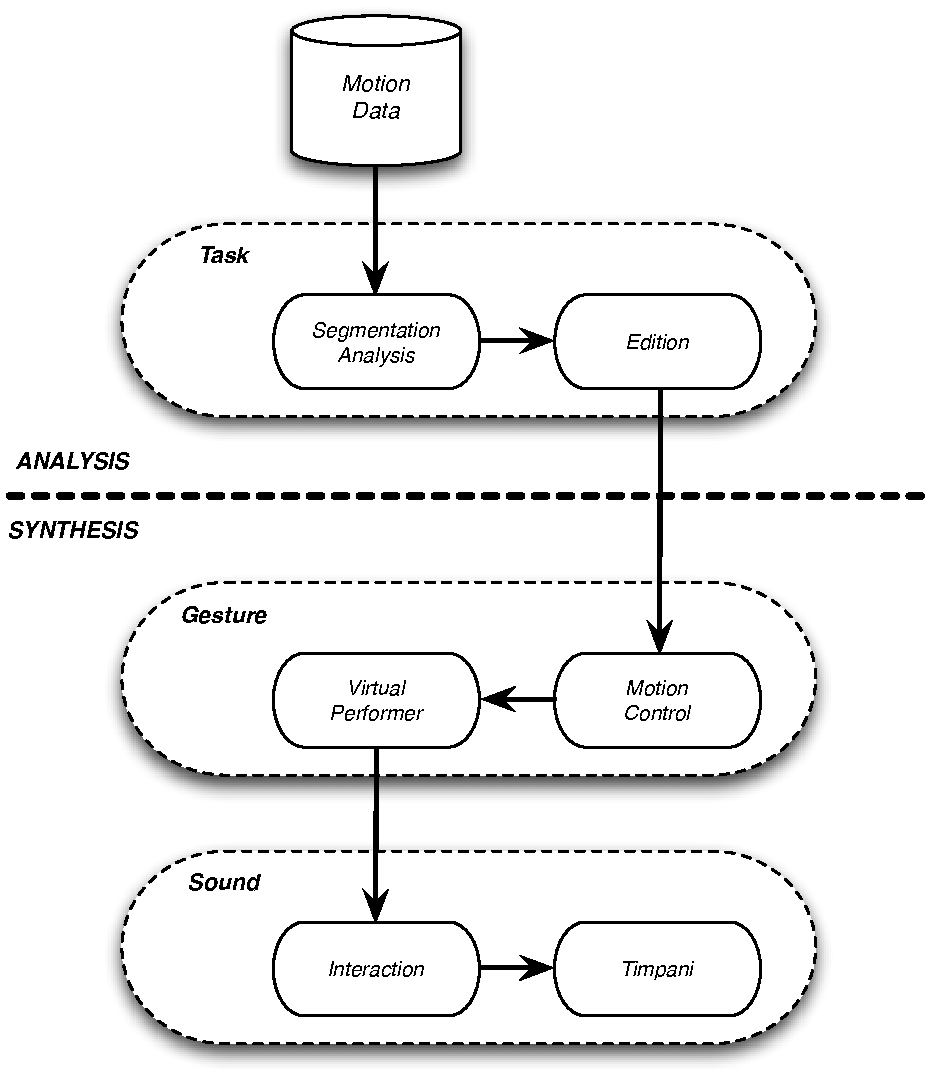
\includegraphics[width=0.75\textwidth]{Chapters/3/Pics/Pdf/GeneralApproach-b&w.pdf}
	\end{center}
	\vspace{-0.5cm}
	\caption[Overview of the approach]{Overview of the approach.}
	\label{fig:thesisOverview}
\end{figure}

%%%%%%%%%%%%%%%%%%%%%%%%%%%%%%%%%%%%%%%%%%%%%%%%%%%%%%%%%%%%%%%%%%%%%%%%%%%%%%%%%%%%%%%%%%%%%%%%%%%%%%%%%%%%%%%%%%%%


%%%%%%%%%%%%%%%%%%%%%%%%%%%%%%%%%%%%%%%%%%%%%%%%%%%%%%%%%%%%%%%%%%%%%%%%%%%%%%%%%%%%%%%%%%%%%%%%%%%%%%%%%%%%%%%%%%%%

	\section{Analysis}
	
One key issue of our work is therefore to finely analyze and understand (see the "Analysis" part in \myfigname \ref{fig:thesisOverview}) the underlying processes involved in the control of the virtual performer, and the way it is related to motion captured data recorded during real performances.\\

In order to achieve these objectives, we highlight in an analysis process the significant dimensions of gesture that are involved when playing various percussion playing techniques. In particular we show that the mallet extremity trajectories may significantly characterize percussion grips as well as playing modes.

Compared to \emph{computer music} methods for \emph{analyzing} instrumental gestures (see section \ref{subsubsec:CM_Control_GC_GAM}), our work differs from the fact that we analyse the influence of various percussion playing techniques on instrumental gestures. We therefore hypothesize that these playing techniques reflect all or part of the expressivity contained in motion. They may be related for instance to the execution speed of movements, different dynamics or types of attacks. We also identify motion parameters for finely representing these playing techniques.\\

Such gesture characteristics may then be used for obtaining a segmented and reduced-dimension representation of motion. The resulting motion chunks may be the basis of an edition and assembling process, in which elementary gesture units are arranged and submitted to the synthesis system for controlling the motion of the virtual performer.

%%%%%%%%%%%%%%%%%%%%%%%%%%%%%%%%%%%%%%%%%%%%%%%%%%%%%%%%%%%%%%%%%%%%%%%%%%%%%%%%%%%%%%%%%%%%%%%%%%%%%%%%%%%%%%%%%%%%


%%%%%%%%%%%%%%%%%%%%%%%%%%%%%%%%%%%%%%%%%%%%%%%%%%%%%%%%%%%%%%%%%%%%%%%%%%%%%%%%%%%%%%%%%%%%%%%%%%%%%%%%%%%%%%%%%%%%

	\section{Synthesis}
	
In order to reproduce the main characteristics of the control exerted on a real instrument, and more specifically the efforts involved in the interaction, we adopt a physics-based approach for modeling both the virtual performer and the sound-synthesis process (see the "Synthesis" part in \myfigname \ref{fig:thesisOverview}).\\

Moreover we provide a new motion control scheme dedicated to percussion gestures for controlling the physics model of the virtual performer.

Among physics-based \emph{computer animation} techniques, our solution comes under the category of \emph{controller-based hybrid} methods (section \ref{subsubsec:CA_MC_Hybrid}). The main difference compared to these related works lies in the fact that our contribution leads to the control of the virtual performer only by specifying end-effector trajectories, \emph{i.e.} mallet extremity trajectories. This control mode is also shown to be consistent as regards to the previous analysis results.

Compared to \emph{computer music} methods for \emph{modeling} instrumental gestures (see section \ref{subsubsec:CM_Control_GC_GAM}), our framework allows to represent not only what occurs during the mechanical interaction between the instrumentist and the instrument, but also the whole gesture production system. It includes a physics-based solution for taking into account the preparatory and the retraction phases that precede and follow the interaction process. Furthermore, our work sensibly differs from those that use the gestural signals directly responsible for the sound production, as we build the physical model that produces these gestural signals.\\

The physics modeling approach adopted in this work is then used for allowing to specify the interaction between the physics model of the virtual percussionist and a physics model of a timpani membrane. The ouput of the gesture synthesis are sent to the timpani model to produce the corresponding sounds, thanks to the identification of kinematic and dynamic features of the gesture attacks. A system architecture is also presented for allowing the real-time interaction between motion and sound synthesis.

%%%%%%%%%%%%%%%%%%%%%%%%%%%%%%%%%%%%%%%%%%%%%%%%%%%%%%%%%%%%%%%%%%%%%%%%%%%%%%%%%%%%%%%%%%%%%%%%%%%%%%%%%%%%%%%%%%%%


%%%%%%%%%%%%%%%%%%%%%%%%%%%%%%%%%%%%%%%%%%%%%%%%%%%%%%%%%%%%%%%%%%%%%%%%%%%%%%%%%%%%%%%%%%%%%%%%%%%%%%%%%%%%%%%%%%%%

	\section{Evaluation}

We then proceed to an extensive evaluation of both the analysis and synthesis modules presented in \myfigname \ref{fig:thesisOverview}.\\

As for the analysis part of our work, we provide a quantitative evaluation of the extracted motion parameters that are used for representing the percussion playing techniques under study. %Such a quantitative analysis is inspired from existing works that have successfully been applied to bowed-string gestures (section \ref{subsubsec:CM_Control_GC_GAM}). 
Compared to works related to the analysis of percussion gestures (section \ref{subsubsec:CM_Control_GC_GAM}), our contribution %however gives a fine identification of these motion parameters for discriminating between playing techniques.\\
proposes a set of motion parameters that can clearly and distinctly classify the various playing techniques.\\

Regarding the synthesis system which is proposed in this thesis, we also provide an extensive evaluation of our control mode. It involves its comparison to classical methods that are traditionally used for physically controlling a virtual character (section \ref{subsubsubsubsec:CA_MC_Physics_Controllers}). We focus especially on the accuracy response of these control modes, particularly for the critical issue in percussion gestures of finely controlling mallet extremity trajectories.\\

Finally, we qualitatively evaluate our global framework for synthesizing percussion performances in a musical perspective. This involves the synthesis of percussion exercises that were proposed by a percussion professor. The same percussion expert has then been asked to judge the overall realism and proficiency of the virtual performer to execute these percussion exercises.

%%%%%%%%%%%%%%%%%%%%%%%%%%%%%%%%%%%%%%%%%%%%%%%%%%%%%%%%%%%%%%%%%%%%%%%%%%%%%%%%%%%%%%%%%%%%%%%%%%%%%%%%%%%%%%%%%%%%


